%% ----------------------------------------------------------------
%% Article.tex
%% ---------------------------------------------------------------- 
\documentclass{ecsarticle}     % Use the Article Style
\graphicspath{{Figures/}}   % Location of your graphics files
\usepackage{natbib}            % Use Natbib style for the refs.
\hypersetup{colorlinks=false}   % Set to false for black/white printing
\input{Definitions}            % Include your abbreviations

\usepackage[nodayofweek]{datetime}
\usepackage{listings}
\usepackage{color}

\usepackage{graphicx}



%% ----------------------------------------------------------------
\begin{document}
%TC:ignore
\frontmatter
\title      {COMP6036: Advanced Machine Learning\\
            Feature Selection Challenge}
      
\addresses  {\deptname\\\univname}
\authors                 {\href{mailto:ajr2g10@ecs.soton.ac.uk}{Ashley J. Robinson}\\\href{mailto:ajr2g10@ecs.soton.ac.uk}{ajr2g10@ecs.soton.ac.uk}}

\date       {\today}
\subject    {}
\keywords   {}
\maketitle
%% ----------------------------------------------------------------


\begin{abstract}
\end{abstract}

%TC:endignore
\mainmatter


\section{Introduction}

Each dataset has been divided in three section for training, validation and test submission.
The final partition labels remain hidden from the development process.
The discrete class labels, $t$, and the classifier outputs, $y$, are described by equation~\eqref{eqn:output}.
Keeping to these output values requires using the thresholding function $\Theta$ in equation~\eqref{eqn:theta}. 
Everything implemented has been developed from scratch for the MATLAB programming language. 


\begin{equation}
	y,t \in \{-1,+1\}
	\label{eqn:output}
\end{equation}

\begin{equation}
	\Theta(a) = \left\{ 
      \begin{array}{l}
         +1,\:a > 0\\
         -1,\:a \leq 0\\
      \end{array} \right.	
	\label{eqn:theta}
\end{equation}

\section{Machine Learning Architecure}

\subsection{Perceptron}


The first attempt at classification was using a simple a preceptron architecture; shown in figure~\ref{fig:slp}.
Capable of producing a linear separation boundary subject to equation~\eqref{eqn:slp} the method serves as starting point for further investigation into the data.
The error discrete error from from the training patterns is calculated using equation~\eqref{eqn:slp_error}.
Equation~\eqref{eqn:slp_mat} expands the method by considering many different training patterns applied to only one set of weights.
The weight vector is trained using the iterative learning rule held in equations~\eqref{eqn:slp_learn_1},~\eqref{eqn:slp_learn_2} and~\eqref{eqn:slp_learn_3}~\citep{info05mackay}.
In practice the offset parameter, $b$, is added to the weight vector and every input pattern is appended with a constant unit feature to allow complete training.

\begin{figure}[ht]
   \centering
    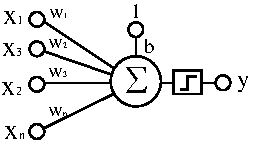
\includegraphics[height = 4cm]{SLP.pdf}
   \caption{Perceptron architecture.}
   \label{fig:slp}
\end{figure}

\begin{equation}
   y = \Theta \left(b + \sum_{i=1}^{n} w_i x_i \right)
   \label{eqn:slp}
\end{equation}

\begin{equation}	
	e = t - y,\:\:e \in \{-2,0.+2\}
	\label{eqn:slp_error}
\end{equation}

\begin{equation}
   \textbf{Y} = \Theta ( \textbf{X}.\textbf{W} + \textbf{b})
   \label{eqn:slp_mat}
\end{equation}

\begin{equation}	
	\textbf{W}_{t+1} = \textbf{W}_t + \Delta \textbf{W}
	\label{eqn:slp_learn_1}
\end{equation}

\begin{equation}	
	\mathbf{E} = (\mathbf{T} - \mathbf{Y})^{T}
	\label{eqn:slp_learn_2}
\end{equation}

\begin{equation}	
	\Delta \mathbf{W} = \mathbf{\eta}*\mathbf{E}\mathbf{X}^T
	\label{eqn:slp_learn_3}
\end{equation}


\subsection{Multi Layer Perceptron}


The first attempt at classification was using a simple a preceptron architecture; shown in figure~\ref{fig:slp}.
Capable of producing a linear separation boundary subject to equation~\eqref{eqn:slp} the method serves as starting point for further investigation into the data.
The error discrete error from from the training patterns is calculated using equation~\eqref{eqn:slp_error}.
Equation~\eqref{eqn:slp_mat} expands the method by considering many different training patterns applied to only one set of weights.
The weight vector is trained using the iterative learning rule held in equations~\eqref{eqn:slp_learn_1},~\eqref{eqn:slp_learn_2} and~\eqref{eqn:slp_learn_3}~\citep{info05mackay}.
In practice the offset parameter, $b$, is added to the weight vector and every input pattern is appended with a constant unit feature to allow complete training.

\begin{figure}[ht]
   \centering
    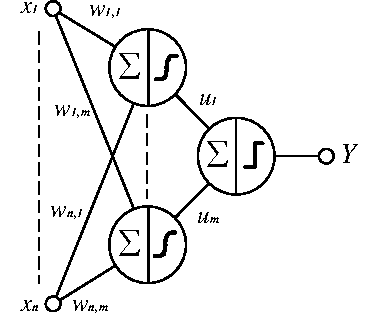
\includegraphics[height = 4cm]{MLP.pdf}
   \caption{Multi Layer Perceptron (MLP) architecture.}
   \label{fig:slp}
\end{figure}

\begin{equation}
   y = \Theta \left(b + \sum_{i=1}^{n} w_i x_i \right)
   \label{eqn:slp}
\end{equation}

\begin{equation}	
	e = t - y,\:\:e \in \{-2,0.+2\}
	\label{eqn:slp_error}
\end{equation}

\begin{equation}
   \textbf{Y} = \Theta ( \textbf{X}.\textbf{W} + \textbf{b})
   \label{eqn:slp_mat}
\end{equation}

\begin{equation}	
	\textbf{W}_{t+1} = \textbf{W}_t + \Delta \textbf{W}
	\label{eqn:slp_learn_1}
\end{equation}

\begin{equation}	
	\mathbf{E} = (\mathbf{T} - \mathbf{Y})^{T}
	\label{eqn:slp_learn_2}
\end{equation}

\begin{equation}	
	\Delta \mathbf{W} = \mathbf{\eta}*\mathbf{E}\mathbf{X}^T
	\label{eqn:slp_learn_3}
\end{equation}



\section{Feature Selection}

\section{Results}

\section{Conclusions}


\newpage

%TC:ignore
\bibliographystyle{ecs}
\bibliography{references}



\backmatter
\begin{appendix}

\newpage
\section{Code Listings}

\end{appendix}

%TC:endignore
\end{document}
%% ----------------------------------------------------------------

